\Section{Analysis- Strategy and Setup}
\label{ch:analysis_strategy}

In this chapter, an overview of the analysis- strategy and setup will be given with a special focus on the physical observable used as the condition for the cINN inference.

\Subsection{Analysis Strategy}

The analysis has been performed on Monte Carlo (MC) data exclusively. The phase space in consideration has been selected to contain the highest signal yield. Hence the $gg \rightarrow WH \rightarrow b\bar{b} l\nu_l$ and $gg \rightarrow ZH \rightarrow b\bar{b}l\bar{l}$ final states have been considered. \textcolor{red}{ The Feynman diagram of these processes are shown in fig. \ref{fig:VH_finalstates}}. Note that due to their weakly-interacting nature, neutrinos cannot be reconstructed in the detector. For this reason, former will be referred to as semi-leptonic and the latter as di-leptonic final state.

\begin{figure}[h!]
	\centering
%	\includegraphics[width=\linewidth]{imagefile}
	\caption{The analysed final states of the $VH$ processes.}
	\label{fig:VH_finalstates}
\end{figure}

The events are categorised through a triggering system and are assigned to four categories. The list of the triggers for the di- and semileptonic channels are listed in tab. \ref{tab:triggers}.

\begin{table}[h!]
	\centering
	\begin{tabular}{cc}
		Channel & Trigger Name \\
		\hline 
		\multirow{2}{*}{$ee$} & \texttt{Ele23\_Ele12\_CaloIdL\_TrackIdL\_IsoVL} \\
		& \texttt{Ele23\_Ele12\_CaloIdL\_TrackIdL\_IsoVL\_DZ} \\
		\hline 
		\multirow{2}{*}{$e$} & \texttt{Ele32\_WPTight\_Gsf} \\
		& \texttt{Ele32\_WPTight\_Gsf\_L1DoubleEG} \\
		\hline 
		\multirow{2}{*}{$\mu\mu$} & \texttt{Mu17\_TrkIsoVVL\_Mu8\_TrkIsoVVL\_DZ} \\
		& \texttt{Mu17\_TrkIsoVVL\_Mu8\_TrkIsoVVL\_DZ\_Mass3p8} \\
		\hline 
		\multirow{2}{*}{$\mu$} & \texttt{IsoMu24\_eta2p1} \\
		& \texttt{IsoMu27} \\
		\hline \\
	\end{tabular}
	\caption{The lepton triggers used in the analysis.}
	\label{tab:triggers}
\end{table}

The naming in \ref{tab:triggers} indicates the phase space which the triggers cut off. In the di-leptonic channels the lepton with the higher energy (the leading lepton) is required to have $p_T > \SI{23}{\giga\electronvolt}$ and $p_T > \SI{17}{\giga\electronvolt}$ for $ee$ and $\mu\mu$, respectively; the sub-leading (the "other") lepton is then required to have $p_T>\SI{12}{\giga\electronvolt}$ and $\SI{8}{\giga\electronvolt}$ for $ee$ and $\mu\mu$, respectively. In the semi-leptonic categories, only electrons with $p_T>\SI{32}{\giga\electronvolt}$ and isolated muons with $\SI{24}{\giga\electronvolt}$ and $|\eta|<2$ and isolated muons with $p_T>\SI{27}{\giga\electronvolt}$ are kept.

In addition to these selection criteria, both the muon tracks have to be isolated in the $\mu\mu$ channel. For the $e$ channel, the tight working point has been selected as trigger efficiency.

The datasets used for the analysis have been simulated with \texttt{PYTHIA} \cite{Sj_strand_2008} and \texttt{HERWIG++} \cite{herwig}. These simulated events not only contain matrix element calcualtion samples, but also the CMS detectors simulations using \texttt{GEANT4} in order to represent the final observed distribtuions accurately \cite{geant1, geant2, geant3}. The list of the signal sample datsets is shown in tab. \ref{tab:signal_datasets}.

\begin{table}[h!]
	\centering
	\begin{tabular}{ccc}
		Dataset Name & N & $\sigma$/pb \\
		\hline
		\texttt{Dataset1} & & \\
	\end{tabular}
	\caption{\textcolor{red}{The signal datasets}}
	\label{tab:signal_datasets}
\end{table}

For the background processes, one distinguishes between the following processes:

\begin{itemize}
	\item[] \texttt{dy}: Drell-Yan-like vector boson production with hadronic initial state radiation. This process has high cross section and yields the same final state (for radiated bottom jets) as the signal. In addition, it also has the same lepton signature. The process is shown in fig. \ref{fig:dy_background}.
	\begin{figure}[h!]
		\centering
		\caption{\textcolor{red}{The Feynman diagram}}
		\label{fig:dy_background}
	\end{figure}
	\item[] $\texttt{t}\bar{\texttt{t}}$: Production of top quark pairs $t\bar{t}$. These quarks decay via $t\rightarrow Wb$ and with the leptonic decay channel of the $W$, this has the same final state as the signal process. This has the second largest background contribution. The corresponding Feynman diagram is shown in fig. \ref{fig:tt_background}.
	\begin{figure}[h!]
		\centering
		\caption{\textcolor{red}{The Feynman diagram}}
		\label{fig:tt_background}
	\end{figure}
	\item[] $\texttt{t}\bar{\texttt{t}}\texttt{V}$: Associated vector boson production in the initial or final states with a $t\bar{t}$ pair. For the top quarks decaying into bottom quarks and the leptonically decaying vector bosons, this yields a final state similar to the signal final state.
	\item[] $\texttt{st}$: Single top quark production. A hadronically decaying top with a QCD-induced bottom jet results in a semileptonic di-bottom state.
	\item[] \texttt{VV}, \texttt{VVV} and $\texttt{t}{\bar{\texttt{t}}}\texttt{VV}$: di- or triboson production with (or without) associated $t\bar{t}$ production. If any of these vector bosons decay hadronically while the other(s) decay leptonically, this results in a semi- or dileptonic di-bottom final state.
	\item[] $\texttt{t}\bar{\texttt{t}}\texttt{VH}$, \texttt{ggH} and \texttt{VBF}: Higgs production channels.
	\item[] \texttt{wjets}: leptonically decaying jet-associated $W$ boson production.
	\item[] \texttt{QCD}: reducible QCD background.
	\item[] \texttt{rare}: rare processes such as four top production.
\end{itemize}

\textcolor{red}{The list of the background samples from the MC simulations are all listed in tab. \ref{tab:bkg_datasets}}.

\begin{table}[h!]
	\centering
	\begin{tabular}{ccc}
		Sample Name & N & $\sigma$/pb \\
		\hline
		\texttt{Dataset2} & & \\
	\end{tabular}
	\caption{\textcolor{red}{List of simulated background samples.}}
	\label{tab:bkg_datasets}
\end{table}

\Subsection{Analysis Setup}

In the following the selected electron, muon and jet final state objects (reconstructed and identified by ParticleFlow) will be described in detail.

The muon selection criteria are listed in tab. \ref{tab:muon_selection}. For the leading muons, a $p_T$-cut of 25 GeV has been required; qualifying subleading muons need to satisfy $p_T>\SI{15}{\giga\electronvolt}$. Furhtermore, muons ought to be identified as tight muons and have to be contained within the tracker, while their impact parameter (IP) geometry being also compatible with the primary vertex (PV). In addition, the IP significance \texttt{sip3d} (defined as the ratio between the uncertainty of the IP and the IP itself) is also restricted to guarantee that these muons originate from the PV. The \texttt{pfRelISO04\_all} parameter cut ensures the isolation of the muons and hence their origin from the PV.

\begin{table}[h!]
	\centering
	\begin{tabular}{c}
		\hline
		\texttt{tightId} \\
		$p_T > \SI{25}{\giga\electronvolt}/\SI{15}{\giga\electronvolt}$ \\
		$|\eta| \leq 2.4$ \\
		$d_{xy} \leq \SI{0.05}{\centi\meter}$ \\
		$d_z \leq \SI{0.1}{\centi\meter}$ \\
		$\texttt{pfRelIso04\_all} \leq 0.15$  \\
		\texttt{sip3d} $\leq 8$ \\
		\hline \\
	\end{tabular}
	\caption{Selection criteria for the muons. The first and the second values correspond to the cuts applied to the leading and sub-leading muons, respectively.}
	\label{tab:muon_selection}
\end{table}

The electron selection criteria is listed in tab. \ref{tab:electron_selection}. The electrons are required to be included in the tracker (through $\eta$) to ensure quality transversal momentum reconstruction. These electrons should also originate from the primary vertex through the impact parameter (IP) cuts $d_i$. Similarly to muons, the IP significance and isolation measures are also restricted. For quality reconstruction, the maximum number of lost hits in the tracker is also limited. As identification efficiency, the 80\% working point (WP80, defined on a Drell-Yang sample) has been chosen.

\begin{table}[h!]
	\centering
	\begin{tabular}{c}
		\hline
		\texttt{MVA WP80} \\
		$p_T > \SI{25}{\giga\electronvolt}/\SI{15}{\giga\electronvolt} $\\
		$|\eta| \leq 2.5$ \\
		$d_{xy} \leq \SI{0.05}{\centi\meter}$ \\
		$d_z \leq \SI{0.1}{\centi\meter}$ \\
		$\texttt{pfRelIso04\_all} \leq 0.15$  \\
		sip3d $\leq 8$ \\
		$\text{lost hits} \leq 1$ \\
		\hline \\
	\end{tabular}
	\caption{Selection criteria for the muons.}
	\label{tab:electron_selection}
\end{table}

For the jets in consideration, the selection criteria in tab. \ref{tab:jet_selection} are applied. For AK8 jets, the transversal momentum selection lies higher than those of the AK4 jets; both jets are required to carry the tight ID. In addition to that, they should be restricted to the region covered by the tracker. Based on the jet selection, the flavour tacking algorithm identifies the bottom jets. For the AK4-tagging, DeepFlavour and for AK8 jets, DeepDoubleX are used.

\begin{table}[h!]
	\centering
	\begin{tabular}{c}
		\hline
		\texttt{tightId} \\
		$p_T > \SI{30}{\giga\electronvolt}/ \SI{70}{\giga\electronvolt}$ \\
		$|\eta| < 2.4$ \\
		\hline
	\end{tabular}
	\caption{Jet selection criteria. For the transversal cuts the first and the second values are applied to the AK4 and AK8 jets, respectively.}
	\label{tab:jet_selection}
\end{table}

\Subsection{\textcolor{red}{Event Categorisation}}

The resulting histogram for each subcategory and process for the DNN scores is shown in fig. \ref{fig:conditions}.

\begin{figure}[h!]
	\centering
	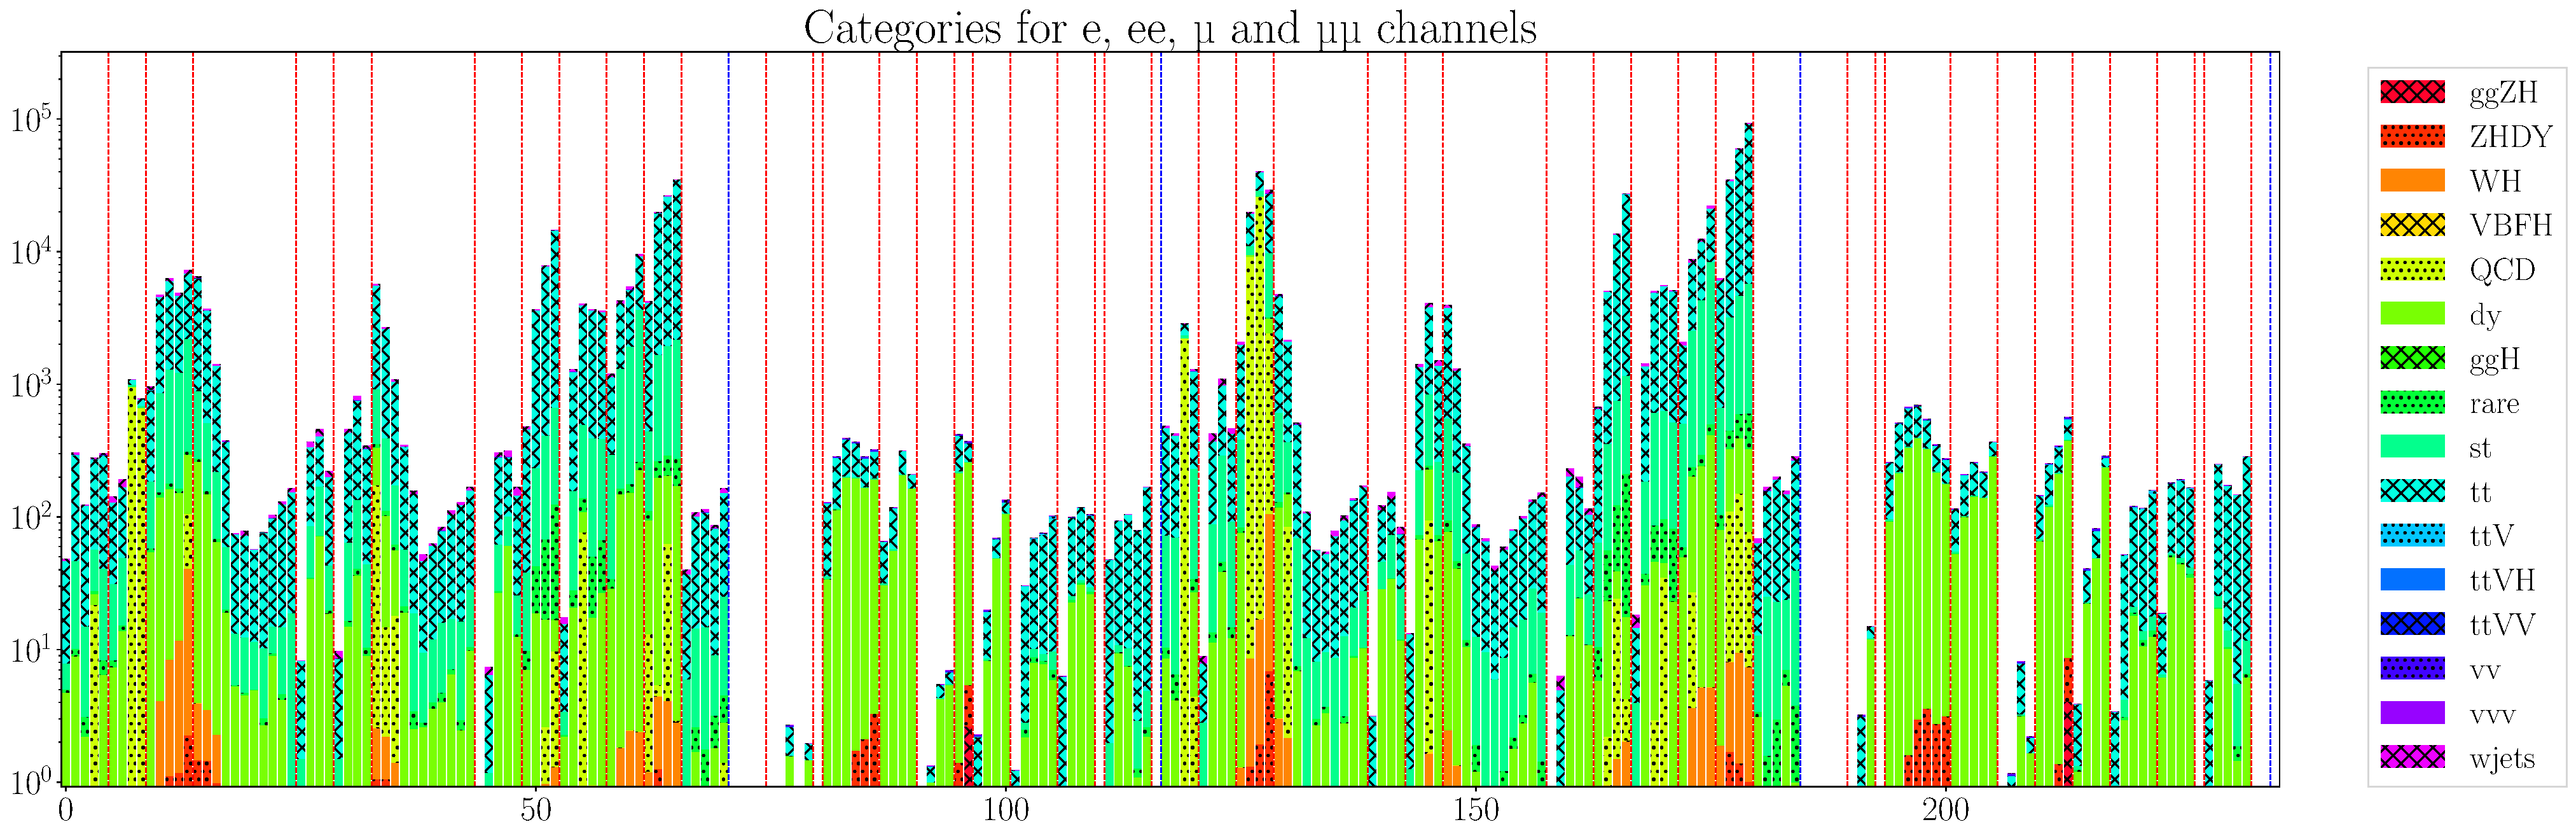
\includegraphics[width=1.1\linewidth]{figures/analysis/cond4_notOrdered.pdf}
	\caption{The distribution of the DNN scores for each subcategory (separated in red) in the semi- and dileptonic categories in consideration (separated in blue). Note the high share of Drell-Yan, $t\bar{t}$ and QCD background events in each bin and the absence of $WH$ events in the dileptonic bins.}
	\label{fig:conditions}
\end{figure}